\documentclass[10pt,a4paper]{article}
\usepackage[latin1]{inputenc}
\usepackage[spanish]{babel}
\usepackage{multicol}
\usepackage{amsmath}
\usepackage{amsfonts}
\usepackage{amssymb}
\usepackage{enumerate}
\usepackage{eurosym}
\usepackage{graphicx}
\usepackage{anysize}
\usepackage{colortbl}
\usepackage{hyperref}
\usepackage{lscape}
\usepackage{float}
\usepackage{longtable}
\usepackage{fancyhdr}
\pagestyle{fancy}
\marginsize{3cm}{2cm}{2cm}{2cm}
\setlength{\parskip}{1em}
\author{Jesus S�nchez-Oro Calvo}
\title{Documento de An�lisis Funcional}
\begin{document}

\thispagestyle{empty}
\begin{center}

\includegraphics[scale=1]{logoURJC.jpg} \\[1cm]
\textbf{\Huge Universidad Rey Juan Carlos}\\[0.5cm]
{\LARGE Escuela T�cnica Superior de Ingenier�a Inform�tica}\\[1.25cm]
{\Large Ingenier�a del Software II}\\[1.25cm]
{\LARGE \textbf{Pr�ctica Obligatoria}}\\[1.25cm]
{\LARGE \textit{Documento de Planificaci�n Final}}\\[2.5cm]
{\Large Radu Tom Vlad \\ David Rufo Valero \\ Jes�s S�nchez-Oro Calvo \\ Adri�n Santalla Romero de �vila }\\[1cm]
{\Large asantalla@siliconkernel.com}\\[2cm]
5� de Ingenier�a Inform�tica \\[1cm]
\today

\end{center}

\newpage
\fancyhead[LO,LE]{Ingenier�a del Software II}
\fancyhead[RO,RE]{Planificaci�n Inicial}
%\fancyfoot[LO,LE]{\thepage}
\tableofcontents

\newpage

\section{Objetivos cumplidos en el desarrollo}
Los objetivos propuestos en la planificaci�n inicial del proyecto han sido satisfechos y comprobados. Por lo tanto, se ha realizado un an�lisis del sistema anterior, mediante el cual se han adaptado necesidades y errores encontrados para a�adirlos al nuevo sistema, obteniendo como resultado el dise�o final del sistema compuesto por el portal de Correos y el portal filat�lico, a falta de la implementaci�n y pruebas de los mismos. En concreto, los resultados de los objetivos pueden verificarse en los siguientes productos:
	\begin{itemize}
	\item \textbf{An�lisis de la funcionalidad disponible en el sistema actual:} Resumen en el Estudio Previo del sistema.
	\item \textbf{Comprobaci�n del sistema actual:} Estudio Previo del sistema
	\item \textbf{Determinaci�n de los elementos nuevos y modificaciones:} Estudio Previo del sistema y documento de An�lisis del sistema.
	\item \textbf{Estudio Previo del sistema:} Documento de estudio previo del sistema
	\item \textbf{An�lisis del sistema:} Documento de an�lisis funcional del sistema
	\item \textbf{Dise�o del sistema:} Documento de dise�o funcional del sistema
	\item \textbf{Prototipo:} Documento de an�lisis funcional del sistema (interfaces), documento de dise�o del sistema (interfaces) y cuaderno de cargas (transferencia de datos)
	\end{itemize}
	
	Con esto quedan cubiertos todos los objetivos iniciales del desarrollo del sistema.

	
\section{Plan de Trabajo Realizado}
El plan de trabajo realizado es el siguiente:
	\begin{figure}[H]
	\begin{center}
	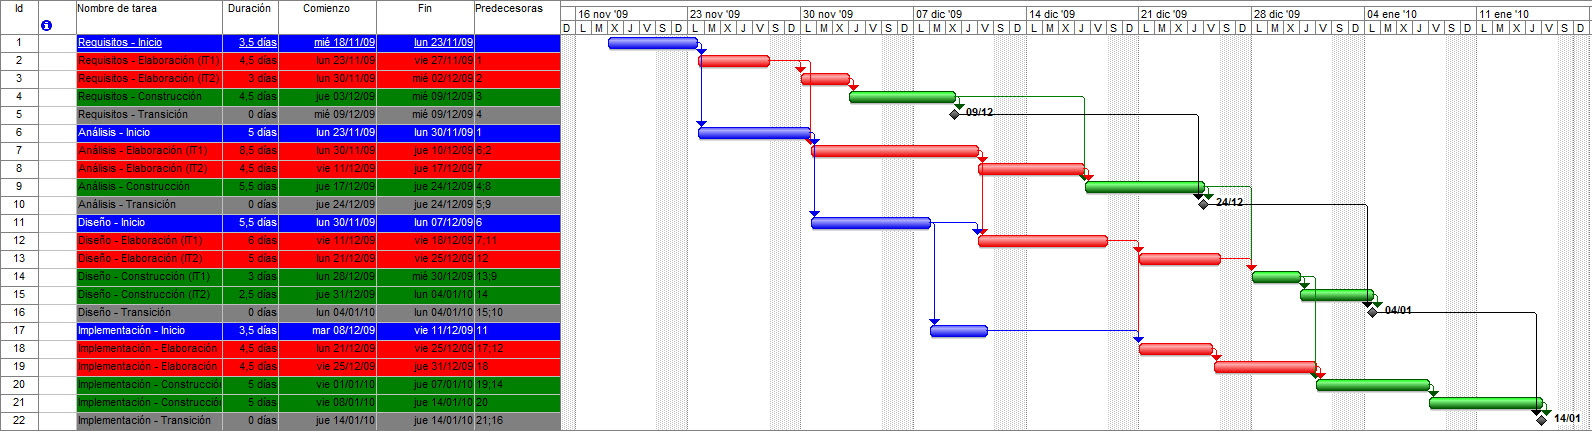
\includegraphics[scale=0.5]{planFin1.jpg}
	\caption{Planificaci�n Final del Sistema}
	\end{center}
	\end{figure}
Como se puede apreciar, se han sufrido diversos retrasos en el desarrollo debido principalmente a la captura de los requisitos, que result� m�s complicada de lo que en un principio pudiera parecer, as� como el desarrollo de un modelo de datos que incluyera todas las funcionalidades necesarias y a la vez fuera funcional. Adem�s, debido a las fechas, con sucesivos festivos, el retraso fue a�n mayor, de un total de un mes aproximadamente.

Por lo tanto, los hitos han sido retrasados de fecha, aunque se producen en el mismo punto de desarrollo que en la planificaci�n inicial.

\end{document}
